\documentclass{beamer}


\mode<presentation>
{
  \usetheme{CambridgeUS}
	\usecolortheme{beaver}
  % or ...

  \setbeamercovered{transparent}
  % or whatever (possibly just delete it)
}


\usepackage{xeCJK}
\usepackage[english]{babel}
\usepackage[utf8]{inputenc}
\usepackage{times}
\usepackage[T1]{fontenc}
\usepackage{hyperref}
\usepackage{pifont}
\usepackage{bibentry}
\usepackage{verbatim}
\usepackage{fontspec}
\newcommand{\cmark}{\ding{51}}%
\newcommand{\xmark}{\ding{55}}%
\setCJKmainfont{WenQuanYi Micro Hei}
\setmainfont{DejaVu Sans}


\title[开源软件基础] 
{开源软件基础}
\subtitle{matplotlib}

\author[Zhilei Ren] 
{Zhilei Ren}

\institute[OSCAR Team] % (optional, but mostly needed)
{
\\
\includegraphics[width=0.2\textwidth]{../../utils/logo.jpg}\\
OSCAR Team, School of Software, 
Dalian University of Technology
}


\subject{Open source software}

\pgfdeclareimage[height=0.5cm]{university-logo}{../../utils/logo.jpg}
\logo{\pgfuseimage{university-logo}}



% Delete this, if you do not want the table of contents to pop up at
% the beginning of each subsection:
\AtBeginSubsection[]
{
  \begin{frame}<beamer>{Outline}
    \tableofcontents[currentsection,currentsubsection]
  \end{frame}
}


% If you wish to uncover everything in a step-wise fashion, uncomment
% the following command: 

%\beamerdefaultoverlayspecification{<+->}

\setbeamertemplate{section in toc}[circle]
\setbeamertemplate{items}[circle]
\setbeamertemplate{caption}[numbered]
\setbeamertemplate{bibliography item}{\insertbiblabel}
\setbeamertemplate{bibliography entry title}{}
\setbeamertemplate{bibliography entry journal}{}

\begin{document}

\begin{frame}
  \titlepage
\end{frame}

\begin{frame}{Outline}
  \tableofcontents[currentsection,currentsubsection, 
    hideothersubsections, 
    sectionstyle=show,
]
\end{frame}

\AtBeginSection[]
{
 \begin{frame}<beamer>
 \frametitle{Outline}
 \tableofcontents[currentsection]
 \end{frame}
}

\begin{frame}
  \frametitle{今天就能开始用的小知识}
	\begin{block}
		{creat}
		Ken Thompson was once asked what he would do differently if he were redesigning the UNIX system. His reply: "I'd spell creat with an e."\footnote{\url{https://en.wikiquote.org/wiki/Ken_Thompson}}
	\end{block}
	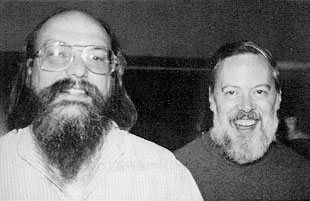
\includegraphics[width=0.3\linewidth]{Ken-dennis.jpg}
\end{frame}
\begin{frame}
  \frametitle{今天就能开始用的小知识}
	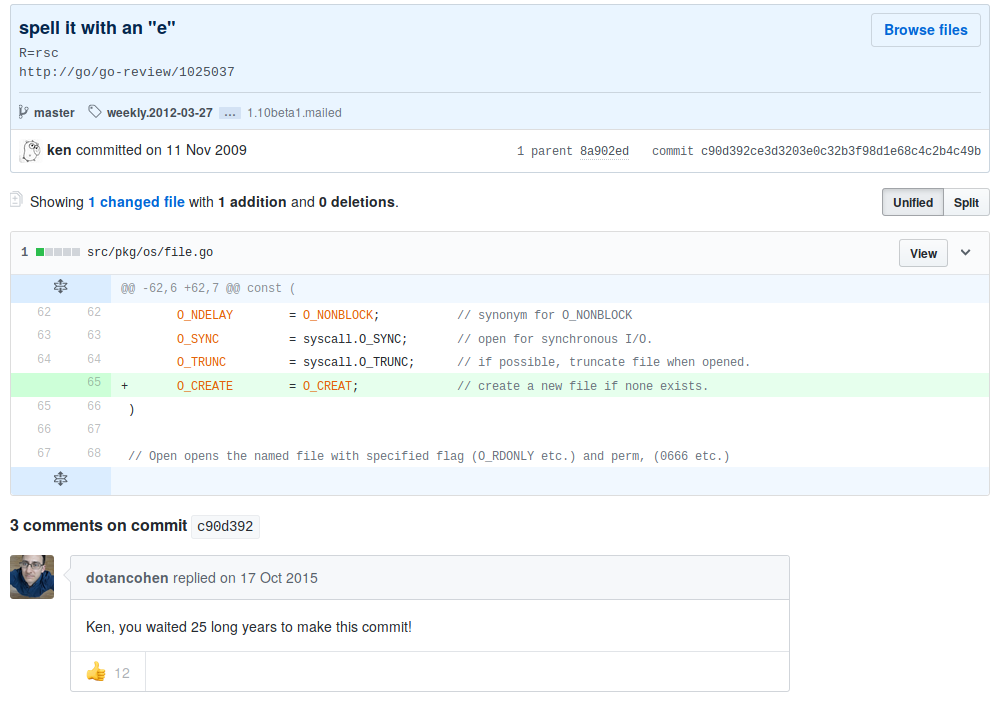
\includegraphics[width=0.8\linewidth]{creat.png}
\end{frame}
\section{Line Plot}


\begin{frame}
  \frametitle{操作步骤}
	
	\begin{itemize}
		\item 使用import numpy引入numpy库
		\item 使用numpy.linspace或numpy.arange或列表准备数据
		\item 使用import matplotlib.pyplot as plt引入包
		\item 使用plt.plot(x, y)和plot.show()画图（推荐jupyter）
		\item 使用plt.xlabel('')，plt.ylabel('')，plt.title('')设置标题
		\item 使用plt.savefig(fname, dpi)保存图片
		\item 使用fig, ax = plt.subplots()返回图片句柄和坐标轴
		\item fig.savefig()保存图片
		\item ax.plot画图
		\item ax.set(xlabel=``x'', ylabel=``y'', title=``title'')
	\end{itemize}
\end{frame}
\begin{frame}[t]{Simple Plot}

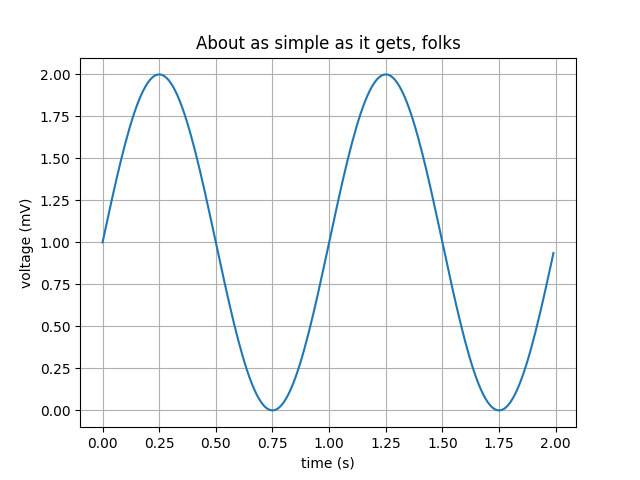
\includegraphics[width=0.8\linewidth]{sphx-glr-simple-plot-001.png}

\end{frame}


\begin{frame}[t,fragile]{Simple Plot}


	\scriptsize
\begin{verbatim}

import matplotlib.pyplot as plt
import numpy as np

# Data for plotting
t = np.arange(0.0, 2.0, 0.01)
s = 1 + np.sin(2 * np.pi * t)

# Note that using plt.subplots below is equivalent to using
# fig = plt.figure and then ax = fig.add_subplot(111)
fig, ax = plt.subplots()
ax.plot(t, s)

ax.set(xlabel='time (s)', ylabel='voltage (mV)',
       title='About as simple as it gets, folks')
ax.grid()

fig.savefig("test.png")
plt.show()


\end{verbatim}


\end{frame}

\section{Histograms}

\begin{frame}[t]{Demo of the histogram (hist) function with a few features}

Selecting different bin counts and sizes can significantly affect the
shape of a histogram. The Astropy docs have a great section on how to
select these parameters:
http://docs.astropy.org/en/stable/visualization/histogram.html

\end{frame}


\begin{frame}[t]{Demo of the histogram (hist) function with a few features}

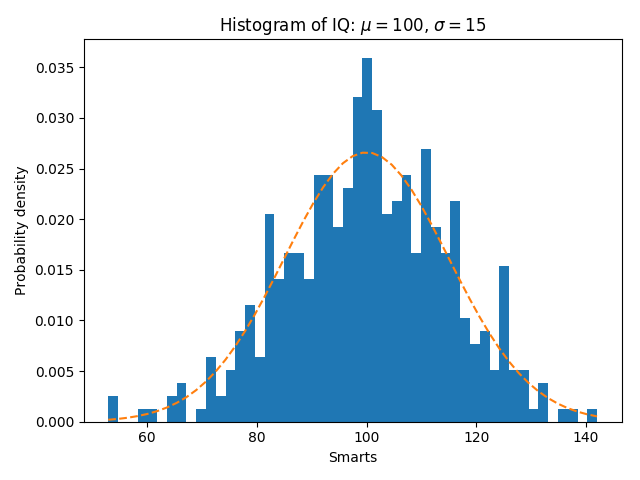
\includegraphics[width=0.8\linewidth]{sphx-glr-histogram-features-001.png}

\end{frame}


\begin{frame}[t,fragile]{Demo of the histogram (hist) function with a few features}


	\scriptsize
\begin{verbatim}
import numpy as np
import matplotlib.pyplot as plt
np.random.seed(19680801)
mu, sigma = 100, 15
x = mu + sigma * np.random.randn(10000)

# the histogram of the data
n, bins, patches = plt.hist(x, 50, normed=1, facecolor='g', alpha=0.75)

plt.xlabel('Smarts')
plt.ylabel('Probability')
plt.title('Histogram of IQ')
plt.axis([40, 160, 0, 0.03])
plt.grid(True)
plt.show()
\end{verbatim}


\end{frame}


%%%%%\section{mplot3d}
%%%%%
%%%%%\begin{frame}[t]{3D surface (color map)}
%%%%%
%%%%%Demonstrates plotting a 3D surface colored with the coolwarm color map.
%%%%%The surface is made opaque by using antialiased=False.
%%%%%
%%%%%\end{frame}
%%%%%
%%%%%
%%%%%\begin{frame}[t]{3D surface (color map)}
%%%%%
%%%%%Also demonstrates using the LinearLocator and custom formatting for the
%%%%%z axis tick labels.
%%%%%
%%%%%\end{frame}
%%%%%
%%%%%
%%%%%\begin{frame}[t]{3D surface (color map)}
%%%%%
%%%%%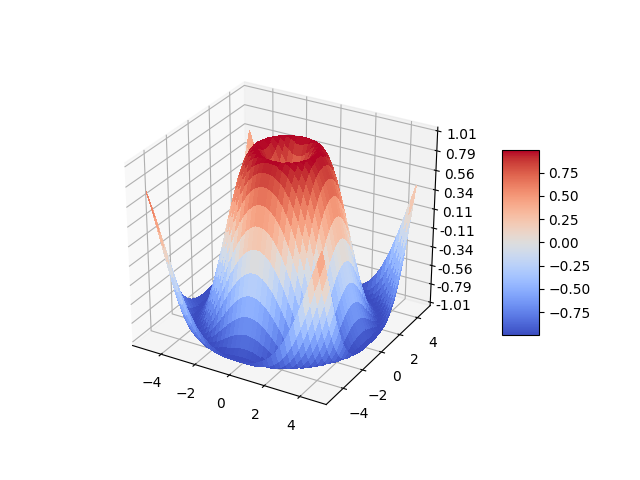
\includegraphics[width=0.8\linewidth]{sphx-glr-surface3d-001.png}
%%%%%
%%%%%\end{frame}
%%%%%
%%%%%
%%%%%\begin{frame}[t,fragile]{3D surface (color map)}
%%%%%
%%%%%
%%%%%	\scriptsize
%%%%%\begin{verbatim}
%%%%%
%%%%%from mpl_toolkits.mplot3d import Axes3D
%%%%%import matplotlib.pyplot as plt
%%%%%from matplotlib import cm
%%%%%from matplotlib.ticker import LinearLocator, FormatStrFormatter
%%%%%import numpy as np
%%%%%fig = plt.figure()
%%%%%ax = fig.gca(projection='3d')
%%%%%
%%%%%# Make data.
%%%%%X = np.arange(-5, 5, 0.25)
%%%%%Y = np.arange(-5, 5, 0.25)
%%%%%X, Y = np.meshgrid(X, Y)
%%%%%R = np.sqrt(X**2 + Y**2)
%%%%%Z = np.sin(R)
%%%%%
%%%%%# Plot the surface.
%%%%%surf = ax.plot_surface(X, Y, Z, cmap=cm.coolwarm,
%%%%%                       linewidth=0, antialiased=False)
%%%%%
%%%%%# Customize the z axis.
%%%%%ax.set_zlim(-1.01, 1.01)
%%%%%ax.zaxis.set_major_locator(LinearLocator(10))
%%%%%ax.zaxis.set_major_formatter(FormatStrFormatter('%.02f'))
%%%%%
%%%%%# Add a color bar which maps values to colors.
%%%%%fig.colorbar(surf, shrink=0.5, aspect=5)
%%%%%
%%%%%plt.show()
%%%%%
%%%%%
%%%%%\end{verbatim}
%%%%%
%%%%%
%%%%%\end{frame}





%%%%%\section{Bar charts}
%%%%%
%%%%%\begin{frame}[t]{Barchart Demo}
%%%%%
%%%%%Bar charts of many shapes and sizes with Matplotlib.
%%%%%
%%%%%\end{frame}
%%%%%
%%%%%
%%%%%\begin{frame}[t]{Barchart Demo}
%%%%%
%%%%%Bar charts are useful for visualizing counts, or summary statistics
%%%%%with error bars. These examples show a few ways to do this with Matplotlib.
%%%%%
%%%%%\end{frame}
%%%%%
%%%%%
%%%%%\begin{frame}[t,fragile]{Barchart Demo}
%%%%%
%%%%%
%%%%%	\scriptsize
%%%%%\begin{verbatim}
%%%%%
%%%%%# Credit: Josh Hemann
%%%%%
%%%%%import numpy as np
%%%%%import matplotlib.pyplot as plt
%%%%%from matplotlib.ticker import MaxNLocator
%%%%%from collections import namedtuple
%%%%%
%%%%%
%%%%%n_groups = 5
%%%%%
%%%%%means_men = (20, 35, 30, 35, 27)
%%%%%std_men = (2, 3, 4, 1, 2)
%%%%%
%%%%%means_women = (25, 32, 34, 20, 25)
%%%%%std_women = (3, 5, 2, 3, 3)
%%%%%
%%%%%fig, ax = plt.subplots()
%%%%%
%%%%%index = np.arange(n_groups)
%%%%%bar_width = 0.35
%%%%%
%%%%%opacity = 0.4
%%%%%error_config = {'ecolor': '0.3'}
%%%%%
%%%%%rects1 = ax.bar(index, means_men, bar_width,
%%%%%                alpha=opacity, color='b',
%%%%%                yerr=std_men, error_kw=error_config,
%%%%%                label='Men')
%%%%%
%%%%%rects2 = ax.bar(index + bar_width, means_women, bar_width,
%%%%%                alpha=opacity, color='r',
%%%%%                yerr=std_women, error_kw=error_config,
%%%%%                label='Women')
%%%%%
%%%%%ax.set_xlabel('Group')
%%%%%ax.set_ylabel('Scores')
%%%%%ax.set_title('Scores by group and gender')
%%%%%ax.set_xticks(index + bar_width / 2)
%%%%%ax.set_xticklabels(('A', 'B', 'C', 'D', 'E'))
%%%%%ax.legend()
%%%%%
%%%%%fig.tight_layout()
%%%%%plt.show()
%%%%%
%%%%%
%%%%%\end{verbatim}
%%%%%
%%%%%
%%%%%\end{frame}
%%%%%
%%%%%
%%%%%\begin{frame}[t]{Barchart Demo}
%%%%%
%%%%%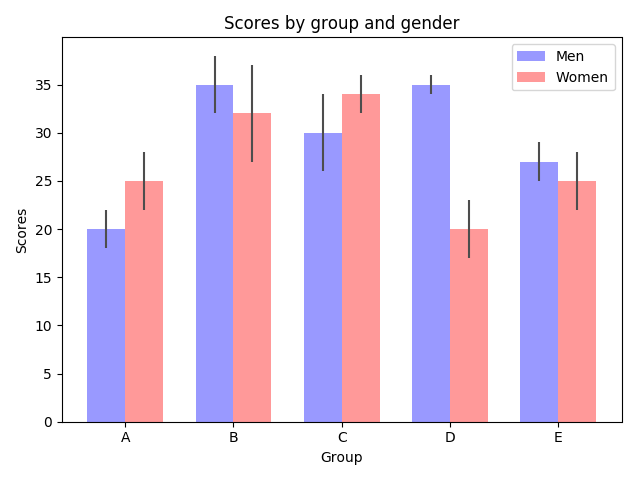
\includegraphics[width=0.8\linewidth]{sphx-glr-barchart-demo-001.png}
%%%%%
%%%%%\end{frame}
%%%%%
%%%%%
%%%%%\begin{frame}[t]{Barchart Demo}
%%%%%
%%%%%This example comes from an application in which grade school gym
%%%%%teachers wanted to be able to show parents how their child did across
%%%%%a handful of fitness tests, and importantly, relative to how other
%%%%%children did. To extract the plotting code for demo purposes, we’ll
%%%%%just make up some data for little Johnny Doe…
%%%%%
%%%%%\end{frame}
%%%%%
%%%%%
%%%%%\begin{frame}[t,fragile]{Barchart Demo}
%%%%%
%%%%%
%%%%%	\scriptsize
%%%%%\begin{verbatim}
%%%%%
%%%%%Student = namedtuple('Student', ['name', 'grade', 'gender'])
%%%%%Score = namedtuple('Score', ['score', 'percentile'])
%%%%%
%%%%%# GLOBAL CONSTANTS
%%%%%testNames = ['Pacer Test', 'Flexed Arm\n Hang', 'Mile Run', 'Agility',
%%%%%             'Push Ups']
%%%%%testMeta = dict(zip(testNames, ['laps', 'sec', 'min:sec', 'sec', '']))
%%%%%
%%%%%
%%%%%def attach_ordinal(num):
%%%%%    """helper function to add ordinal string to integers
%%%%%
%%%%%    1 -> 1st
%%%%%    56 -> 56th
%%%%%    """
%%%%%    suffixes = dict((str(i), v) for i, v in
%%%%%                    enumerate(['th', 'st', 'nd', 'rd', 'th',
%%%%%                               'th', 'th', 'th', 'th', 'th']))
%%%%%
%%%%%    v = str(num)
%%%%%    # special case early teens
%%%%%    if v in {'11', '12', '13'}:
%%%%%        return v + 'th'
%%%%%    return v + suffixes[v[-1]]
%%%%%
%%%%%
%%%%%def format_score(scr, test):
%%%%%    """
%%%%%    Build up the score labels for the right Y-axis by first
%%%%%    appending a carriage return to each string and then tacking on
%%%%%    the appropriate meta information (i.e., 'laps' vs 'seconds'). We
%%%%%    want the labels centered on the ticks, so if there is no meta
%%%%%    info (like for pushups) then don't add the carriage return to
%%%%%    the string
%%%%%    """
%%%%%    md = testMeta[test]
%%%%%    if md:
%%%%%        return '{0}\n{1}'.format(scr, md)
%%%%%    else:
%%%%%        return scr
%%%%%
%%%%%
%%%%%def format_ycursor(y):
%%%%%    y = int(y)
%%%%%    if y < 0 or y >= len(testNames):
%%%%%        return ''
%%%%%    else:
%%%%%        return testNames[y]
%%%%%
%%%%%
%%%%%def plot_student_results(student, scores, cohort_size):
%%%%%    #  create the figure
%%%%%    fig, ax1 = plt.subplots(figsize=(9, 7))
%%%%%    fig.subplots_adjust(left=0.115, right=0.88)
%%%%%    fig.canvas.set_window_title('Eldorado K-8 Fitness Chart')
%%%%%
%%%%%    pos = np.arange(len(testNames))
%%%%%
%%%%%    rects = ax1.barh(pos, [scores[k].percentile for k in testNames],
%%%%%                     align='center',
%%%%%                     height=0.5, color='m',
%%%%%                     tick_label=testNames)
%%%%%
%%%%%    ax1.set_title(student.name)
%%%%%
%%%%%    ax1.set_xlim([0, 100])
%%%%%    ax1.xaxis.set_major_locator(MaxNLocator(11))
%%%%%    ax1.xaxis.grid(True, linestyle='--', which='major',
%%%%%                   color='grey', alpha=.25)
%%%%%
%%%%%    # Plot a solid vertical gridline to highlight the median position
%%%%%    ax1.axvline(50, color='grey', alpha=0.25)
%%%%%    # set X-axis tick marks at the deciles
%%%%%    cohort_label = ax1.text(.5, -.07, 'Cohort Size: {0}'.format(cohort_size),
%%%%%                            horizontalalignment='center', size='small',
%%%%%                            transform=ax1.transAxes)
%%%%%
%%%%%    # Set the right-hand Y-axis ticks and labels
%%%%%    ax2 = ax1.twinx()
%%%%%
%%%%%    scoreLabels = [format_score(scores[k].score, k) for k in testNames]
%%%%%
%%%%%    # set the tick locations
%%%%%    ax2.set_yticks(pos)
%%%%%    # make sure that the limits are set equally on both yaxis so the
%%%%%    # ticks line up
%%%%%    ax2.set_ylim(ax1.get_ylim())
%%%%%
%%%%%    # set the tick labels
%%%%%    ax2.set_yticklabels(scoreLabels)
%%%%%
%%%%%    ax2.set_ylabel('Test Scores')
%%%%%
%%%%%    ax2.set_xlabel(('Percentile Ranking Across '
%%%%%                    '{grade} Grade {gender}s').format(
%%%%%                        grade=attach_ordinal(student.grade),
%%%%%                        gender=student.gender.title()))
%%%%%
%%%%%    rect_labels = []
%%%%%    # Lastly, write in the ranking inside each bar to aid in interpretation
%%%%%    for rect in rects:
%%%%%        # Rectangle widths are already integer-valued but are floating
%%%%%        # type, so it helps to remove the trailing decimal point and 0 by
%%%%%        # converting width to int type
%%%%%        width = int(rect.get_width())
%%%%%
%%%%%        rankStr = attach_ordinal(width)
%%%%%        # The bars aren't wide enough to print the ranking inside
%%%%%        if (width < 5):
%%%%%            # Shift the text to the right side of the right edge
%%%%%            xloc = width + 1
%%%%%            # Black against white background
%%%%%            clr = 'black'
%%%%%            align = 'left'
%%%%%        else:
%%%%%            # Shift the text to the left side of the right edge
%%%%%            xloc = 0.98*width
%%%%%            # White on magenta
%%%%%            clr = 'white'
%%%%%            align = 'right'
%%%%%
%%%%%        # Center the text vertically in the bar
%%%%%        yloc = rect.get_y() + rect.get_height()/2.0
%%%%%        label = ax1.text(xloc, yloc, rankStr, horizontalalignment=align,
%%%%%                         verticalalignment='center', color=clr, weight='bold',
%%%%%                         clip_on=True)
%%%%%        rect_labels.append(label)
%%%%%
%%%%%    # make the interactive mouse over give the bar title
%%%%%    ax2.fmt_ydata = format_ycursor
%%%%%    # return all of the artists created
%%%%%    return {'fig': fig,
%%%%%            'ax': ax1,
%%%%%            'ax_right': ax2,
%%%%%            'bars': rects,
%%%%%            'perc_labels': rect_labels,
%%%%%            'cohort_label': cohort_label}
%%%%%
%%%%%student = Student('Johnny Doe', 2, 'boy')
%%%%%scores = dict(zip(testNames,
%%%%%                  (Score(v, p) for v, p in
%%%%%                   zip(['7', '48', '12:52', '17', '14'],
%%%%%                       np.round(np.random.uniform(0, 1,
%%%%%                                                  len(testNames))*100, 0)))))
%%%%%cohort_size = 62  # The number of other 2nd grade boys
%%%%%
%%%%%arts = plot_student_results(student, scores, cohort_size)
%%%%%plt.show()
%%%%%
%%%%%
%%%%%\end{verbatim}
%%%%%
%%%%%
%%%%%\end{frame}
%%%%%
%%%%%
%%%%%\begin{frame}[t]{Barchart Demo}
%%%%%
%%%%%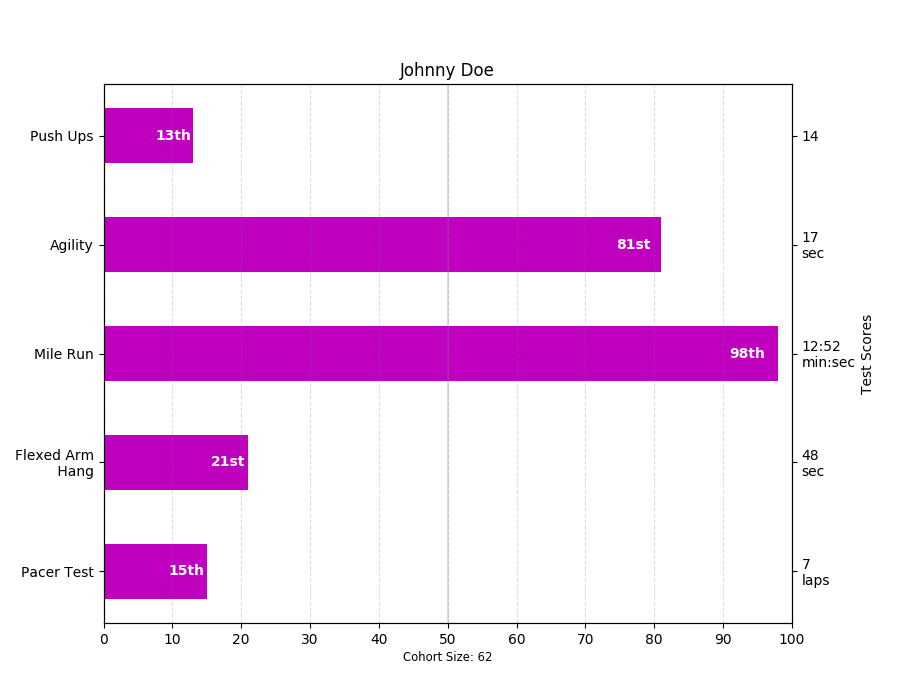
\includegraphics[width=0.8\linewidth]{sphx-glr-barchart-demo-002.png}
%%%%%
%%%%%\end{frame}
%%%%%
%%%%%
%%%%%
%%%%%
%%%%%
\section{Pie charts}

\begin{frame}[t]{Basic pie chart}

Demo of a basic pie chart plus a few additional features.

\end{frame}


\begin{frame}[t]{Basic pie chart}

In addition to the basic pie chart, this demo shows a few optional features:

\end{frame}


\begin{frame}[t]{Basic pie chart}

Note about the custom start angle:

\end{frame}


\begin{frame}[t]{Basic pie chart}

The default startangle is 0, which would start the “Frogs” slice on the
positive x-axis. This example sets startangle = 90 such that everything is
rotated counter-clockwise by 90 degrees, and the frog slice starts on the
positive y-axis.

\end{frame}


\begin{frame}[t]{Basic pie chart}

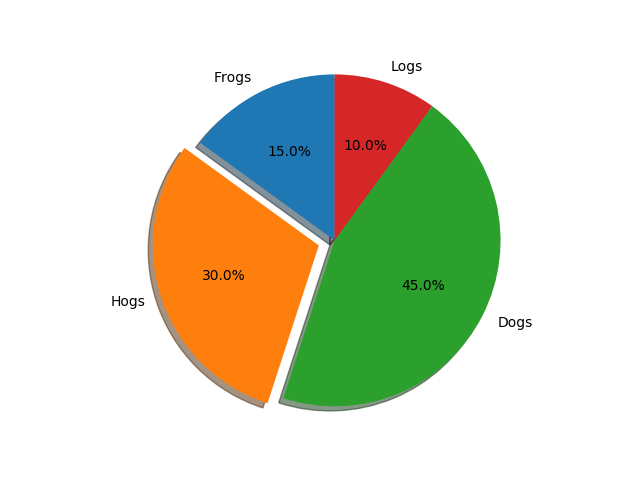
\includegraphics[width=0.8\linewidth]{sphx-glr-pie-features-001.png}

\end{frame}


\begin{frame}[t,fragile]{Basic pie chart}


	\scriptsize
\begin{verbatim}

import matplotlib.pyplot as plt

# Pie chart, where the slices will be ordered and plotted counter-clockwise:
labels = 'Frogs', 'Hogs', 'Dogs', 'Logs'
sizes = [15, 30, 45, 10]
explode = (0, 0.1, 0, 0)  # only "explode" the 2nd slice (i.e. 'Hogs')

fig1, ax1 = plt.subplots()
ax1.pie(sizes, explode=explode, labels=labels, autopct='%1.1f%%',
        shadow=True, startangle=90)
ax1.axis('equal')  # Equal aspect ratio ensures that pie is drawn as a circle.

plt.show()


\end{verbatim}


\end{frame}







\section{Fill demo}

\begin{frame}[t]{Fill plot demo}

Demo fill plot.

\end{frame}


\begin{frame}[t,fragile]{Fill plot demo}


	\scriptsize
\begin{verbatim}

import numpy as np
import matplotlib.pyplot as plt

x = np.linspace(0, 1, 500)
y = np.sin(4 * np.pi * x) * np.exp(-5 * x)
\end{verbatim}


\end{frame}

\begin{frame}[t,fragile]{Fill plot demo}
	\scriptsize
\begin{verbatim}
fig, ax = plt.subplots()

ax.fill(x, y, zorder=10)
ax.grid(True, zorder=5)

x = np.linspace(0, 2 * np.pi, 500)
y1 = np.sin(x)
y2 = np.sin(3 * x)


\end{verbatim}
\end{frame}


\begin{frame}[t]{Fill plot demo}

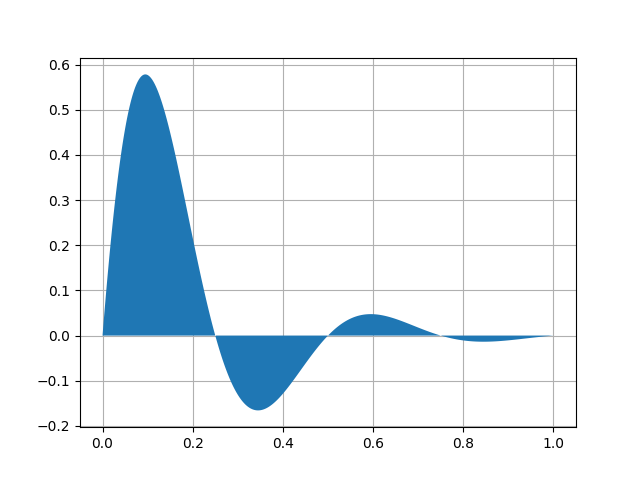
\includegraphics[width=0.8\linewidth]{sphx-glr-fill-001.png}

\end{frame}

\section{Log plots}

\begin{frame}[t]{Log Demo}

Examples of plots with logarithmic axes.

\end{frame}


\begin{frame}[t]{Log Demo}

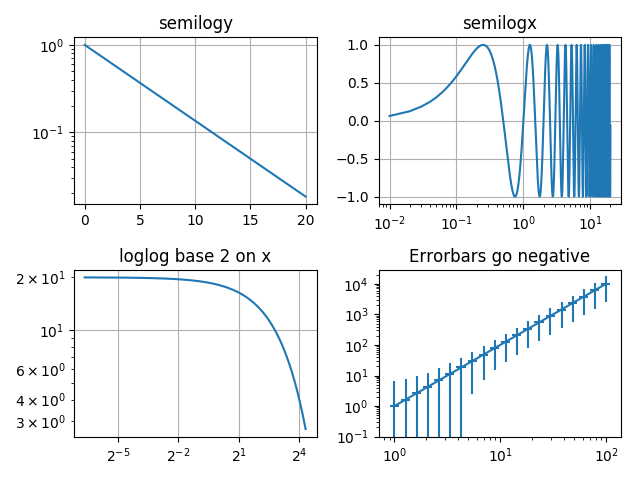
\includegraphics[width=0.8\linewidth]{sphx-glr-log-demo-001.png}

\end{frame}


\begin{frame}[t,fragile]{Log Demo}


	\scriptsize
\begin{verbatim}

import numpy as np
import matplotlib.pyplot as plt

# Data for plotting
t = np.arange(0.01, 20.0, 0.01)

# Create figure
fig, ((ax1, ax2), (ax3, ax4)) = plt.subplots(2, 2)

# log y axis
ax1.semilogy(t, np.exp(-t / 5.0))
ax1.set(title='semilogy')
ax1.grid()

# log x axis
ax2.semilogx(t, np.sin(2 * np.pi * t))
ax2.set(title='semilogx')
ax2.grid()

# log x and y axis
ax3.loglog(t, 20 * np.exp(-t / 10.0), basex=2)
ax3.set(title='loglog base 2 on x')
ax3.grid()

# With errorbars: clip non-positive values
# Use new data for plotting
x = 10.0**np.linspace(0.0, 2.0, 20)
y = x**2.0

ax4.set_xscale("log", nonposx='clip')
ax4.set_yscale("log", nonposy='clip')
ax4.set(title='Errorbars go negative')
ax4.errorbar(x, y, xerr=0.1 * x, yerr=5.0 + 0.75 * y)
# ylim must be set after errorbar to allow errorbar to autoscale limits
ax4.set_ylim(ymin=0.1)

fig.tight_layout()
plt.show()


\end{verbatim}


\end{frame}





%\section{Polar plots}
%
%\begin{frame}[t]{Polar Demo}
%
%Demo of a line plot on a polar axis.
%
%\end{frame}
%
%
%\begin{frame}[t]{Polar Demo}
%
%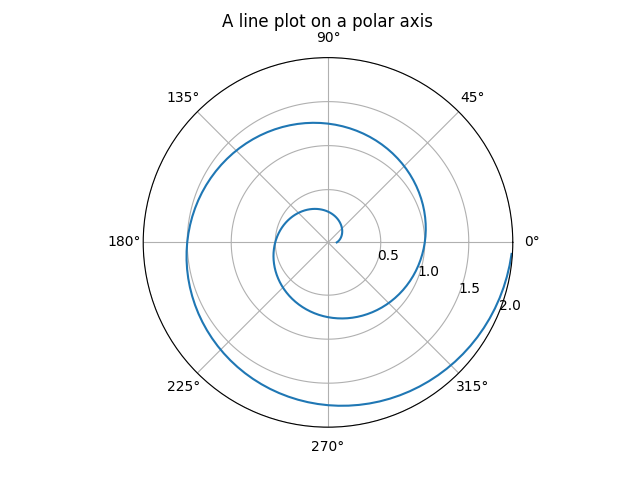
\includegraphics[width=0.8\linewidth]{sphx-glr-polar-demo-001.png}
%
%\end{frame}
%
%
%\begin{frame}[t,fragile]{Polar Demo}
%
%
%	\scriptsize
%\begin{verbatim}
%
%import numpy as np
%import matplotlib.pyplot as plt
%
%
%r = np.arange(0, 2, 0.01)
%theta = 2 * np.pi * r
%
%ax = plt.subplot(111, projection='polar')
%ax.plot(theta, r)
%ax.set_rmax(2)
%ax.set_rticks([0.5, 1, 1.5, 2])  # Less radial ticks
%ax.set_rlabel_position(-22.5)  # Move radial labels away from plotted line
%ax.grid(True)
%
%ax.set_title("A line plot on a polar axis", va='bottom')
%plt.show()
%
%
%\end{verbatim}
%
%
%\end{frame}
%
%
%
%
%
\section{Legends}

\begin{frame}[t]{Legend using pre-defined labels}

Notice how the legend labels are defined with the plots!

\end{frame}


\begin{frame}[t]{Legend using pre-defined labels}

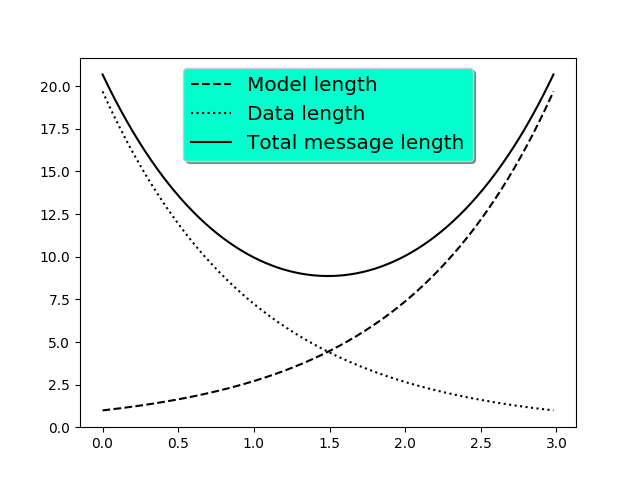
\includegraphics[width=0.8\linewidth]{sphx-glr-legend-001.png}

\end{frame}


\begin{frame}[t,fragile]{Legend using pre-defined labels}


	\scriptsize
\begin{verbatim}

import numpy as np
import matplotlib.pyplot as plt

# Make some fake data.
a = b = np.arange(0, 3, .02)
c = np.exp(a)
d = c[::-1]

# Create plots with pre-defined labels.
fig, ax = plt.subplots()
ax.plot(a, c, 'k--', label='Model length')
ax.plot(a, d, 'k:', label='Data length')
ax.plot(a, c + d, 'k', label='Total message length')

legend = ax.legend(loc='upper center', shadow=True, fontsize='x-large')

# Put a nicer background color on the legend.
legend.get_frame().set_facecolor('#00FFCC')

plt.show()


\end{verbatim}


\end{frame}





\section{XKCD-style sketch plots}

\begin{frame}[t]{XKCD}

Shows how to create an xkcd-like plot.

\end{frame}


\begin{frame}[t]{XKCD}

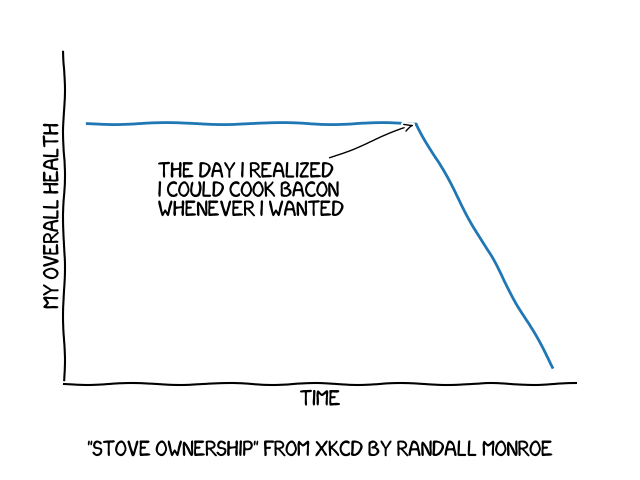
\includegraphics[width=0.8\linewidth]{sphx-glr-xkcd-001.png}

\end{frame}


\begin{frame}[t]{XKCD}

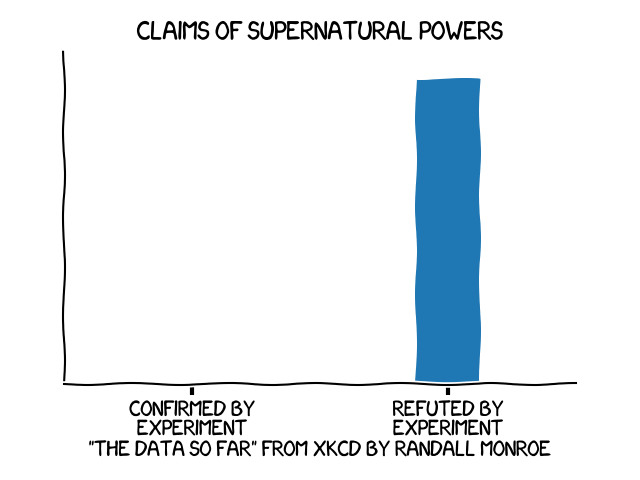
\includegraphics[width=0.8\linewidth]{sphx-glr-xkcd-002.png}

\end{frame}


\begin{frame}[t,fragile]{XKCD}


	\scriptsize
\begin{verbatim}

import matplotlib.pyplot as plt
import numpy as np

with plt.xkcd():
    # Based on "Stove Ownership" from XKCD by Randall Monroe
    # http://xkcd.com/418/

    fig = plt.figure()
    ax = fig.add_axes((0.1, 0.2, 0.8, 0.7))
    ax.spines['right'].set_color('none')
    ax.spines['top'].set_color('none')
    plt.xticks([])
    plt.yticks([])
    ax.set_ylim([-30, 10])

    data = np.ones(100)
    data[70:] -= np.arange(30)

    plt.annotate(
        'THE DAY I REALIZED\nI COULD COOK BACON\nWHENEVER I WANTED',
        xy=(70, 1), arrowprops=dict(arrowstyle='->'), xytext=(15, -10))

    plt.plot(data)

    plt.xlabel('time')
    plt.ylabel('my overall health')
    fig.text(
        0.5, 0.05,
        '"Stove Ownership" from xkcd by Randall Monroe',
        ha='center')

    # Based on "The Data So Far" from XKCD by Randall Monroe
    # http://xkcd.com/373/

    fig = plt.figure()
    ax = fig.add_axes((0.1, 0.2, 0.8, 0.7))
    ax.bar([0, 1], [0, 100], 0.25)
    ax.spines['right'].set_color('none')
    ax.spines['top'].set_color('none')
    ax.xaxis.set_ticks_position('bottom')
    ax.set_xticks([0, 1])
    ax.set_xlim([-0.5, 1.5])
    ax.set_ylim([0, 110])
    ax.set_xticklabels(['CONFIRMED BY\nEXPERIMENT', 'REFUTED BY\nEXPERIMENT'])
    plt.yticks([])

    plt.title("CLAIMS OF SUPERNATURAL POWERS")

    fig.text(
        0.5, 0.05,
        '"The Data So Far" from xkcd by Randall Monroe',
        ha='center')

plt.show()


\end{verbatim}


\end{frame}








\end{document}
